%---------------------------------------------------------------
\chapter{Introduction}
%---------------------------------------------------------------
\setcounter{page}{1}

\section{Motivation, Focus of Thesis}

Theory of finite automata is an important part of computer science curriculum at FIT CTU in Prague and other universities around the world. And although there is a lot of resources one can learn from, there is a lack of those that utilize modern tools. One of such modern tools is iPad (and touch devices in general). This thesis will fill in this gap and build a finite automata editor native application for iPad in this thesis.

Furthermore, I will expand on the recent work done at FIT CTU in Prague concerning development of algorithms library and, more importantly for this thesis, finite automata algorithms including simulating input. This library is named \href{https://alt.fit.cvut.cz/}{Algorithms Library Toolkit} (ALT) \cite{alt} and it has been open sourced.

The main motivation of this thesis is to improve how students learn finite automata and more specifically, enhance the current course BI-AAG that is taught at FIT CTU in Prague. It is also an opportunity to try out algorithms library in practice and create a concrete example of how it can be leveraged.

\section{Thesis Goals}

The main goal of this thesis is to implement a prototype of an automata editor for iPad. This application should enable users to create and edit finite automata with emphasis on touch-based input.
I will also study the web interface of ALT \cite{state-maker} \cite{web-alt}, ALT itself focusing on design and drawing of finite automata, the possibilities of strokes detection on touch devices, and the approaches of shape detection, especially those used in automata drawing on iOS platform.

After the initial study of current approaches, I will implement a prototype of a finite automata editor iPad app that will be capable of finite automata recognition from strokes.

I will then conduct usability testing to assess the usability and shortcomings of the prototype.

\section{Thesis Structure}

Let me now introduce you to the structure of the rest of the thesis:

\begin{itemize}
\item In \textbf{Chapter 2} I will go over the theoretical concepts to properly explain terms and concepts on which it will be built upon later.

\item \textbf{Chapter 3} is concerned with analysis of already existing solutions of creating automata editor, the existing ALT web interface and ALT itself.

\item \textbf{Chapter 4} is about the design of the editor itself.

\item In \textbf{Chapter 5} I will write about the implementation.

\item \textbf{Chapter 6} will go into the specifics of user testing and its outcomes.

\item \textbf{Conclusion} is the last chapter of this thesis.

\end{itemize}

\chapter{Theory}
\label{chap:theory}

Firstly,  I will need to define terms and formal definitions concerning mainly finite automata theory, as that is the main subject of this thesis, and then machine learning as some of its concepts were important during the implementation. 

\section{Formal Languages and Grammars}
 
The following definitions are taken from Automata and Grammars by Eliška Šestáková \cite{automata-and-grammars}, Introduction to Automata Theory, Languages, and Computation \cite{introduction-automata}, and materials from BIE-AAG course \cite{lectures}.

\subsection{Formal Languages}

\begin{definition}
Alphabet (conventionally denoted by $\Sigma$) is a finite set whose elements are called symbols.
\end{definition}
Alphabets therefore can be:
\begin{itemize}
    \item $\Sigma$ = \{0, 1\}
    \item $\Sigma$ = \{a, b, c, d, e\}
    \item $\Sigma$ = \{one, two\}
\end{itemize}

\begin{definition}
String (word) over an alphabet is a finite sequence of symbols from that alphabet.
\end{definition}
\begin{itemize}
    \item $\epsilon$ - \textit{empty string} (string with zero occurences of symbols)
    \item $\Sigma^{*}$ - set of all strings over $\Sigma$
    \item $\Sigma^{+}$ - set of all nonempty strings over $\Sigma$
\end{itemize}
For a binary alphabet $\Sigma$ = \{0, 1\} $\epsilon$, 1001, 100, 1, 001 are all strings over the alphabet $\Sigma$.

\begin{definition}
Formal language L over an alphabet $\Sigma$ is any subset of all the strings over $\Sigma$ - i.e., $L \subseteq \Sigma$
\end{definition}
For a binary alphabet $\Sigma$ = \{0, 1\} a formal language over $\Sigma$ are then subsets of \textit{all} binary strings. We can denote the language either by:
\begin{itemize}
    \item enumeration notation where all possible strings in the language are listed, e.g.: $\textit{L}_1 = \{\epsilon\}, \textit{L}_2 = \{1\}, \textit{L}_3 = \{0, 00, 000, 01\}$ 
    \item set-builder notation where the languages are described in the following way: \{ w $\mid$ something about w \}. Examples are: $\textit{L}_4 = \{\textit{w} \mid \textit{w} \in {0,1}^* \wedge \left|\textit{w}\right| mod 2 = 0\}$, $\textit{L}_5 = \{0^\textit{n}1^\textit{n} : \textit{n} \in \mathbb{N}_0\}$
\end{itemize}

\subsection{Grammar}

Grammars are used to describe languages. Below you can find how they are defined:

\begin{definition}
    \textit{Grammar} is a quadruple of G = (N, $\Sigma$, P, S) where:
\end{definition}
\begin{itemize}
    \item \textit{N} is a finite non-empty set of nonterminal symbols
    \item $\Sigma$ is a finite set of terminal symbols ($\Sigma$ $\cap$ \textit{N} = $\emptyset$). Note that \textit{N} $\cap$ $\Sigma$ = $\emptyset$
    \item \textit{P} is a finite set of \textit{production rules}, assuming the following form:\\

    \centerline{$\alpha\textit{A}\beta \rightarrow \gamma$ ($\alpha, \beta, \gamma \in (\textit{N} \cup \Sigma)^*$)}
\end{itemize}

The following is an example of a grammar that describes the language \textit{L} = $\{01^\textit{n}0 : \textit{n} \in \mathbb{N}_0\}$:
Grammar \textit{G} = (\{\textit{A}, \textit{S}\}, \{0, 1\}, \textit{P}, \textit{S}) where \textit{P}:
\begin{itemize}
    \item \textit{S} $\rightarrow$ 0\textit{A}
    \item \textit{A} $\rightarrow$ 1\textit{A}
    \item \textit{A} $\rightarrow$ 0
\end{itemize}

\subsection{Chomsky Classification of Grammars}

Grammars are divided into four classes where they differ in their production rules. 

\begin{definition}
    Let G = (N, $\Sigma$, P, S). We say that G is:
\end{definition}
\begin{enumerate}
    \item \textit{Unrestricted grammar} (type 0), if every rule is in the form of:
    
    \centerline{$\alpha\textit{A}\beta \rightarrow \gamma$ ($\alpha, \beta, \gamma \in (\textit{N} \cup \Sigma)^*$, $\textit{A} \in \textit{N}$)}
    \item \textit{Context-sensitive} (type 1), if every rule is in the form of:

    \centerline{$\gamma\textit{A}\delta \rightarrow \gamma\alpha\delta$ ($\gamma, \delta \in (\textit{N} \cup \Sigma)^*$, $\textit{a} \in (\textit{N} \cup \Sigma)^+$)}
    or in the form of $\textit{S} \rightarrow \epsilon$ if \textit{S} is not present on the right hand side of any rule of a given grammar.
    \item \textit{Context-free grammar} (type 2) if every rule is in the form of:

    \centerline{$\textit{A} \rightarrow \alpha$ $(\textit{A} \in \textit{N}, \alpha \in (N \cup \Sigma)^*)$}
    \item \textit{Regular grammar} (type 3), if every rule is in the form of:

    \centerline{$\textit{A} \rightarrow \textit{a}$ or $\textit{A} \rightarrow \textit{aB}$ $(\textit{a} \in \Sigma, \textit{A}, \textit{B} \in \textit{N})$}
    or in the form of $\textit{S} \rightarrow \epsilon$ if \textit{S} is not present on the right hand side of any rule of a given grammar.
\end{enumerate}

\subsection{Classification of Languages}
Classification of languages, also known as the Chomsky hierarchy, has the following definition:
\begin{definition}
    We say that language is:
\end{definition}
\begin{enumerate}
    \item \textit{formal} if it is a formal language but is neither regular, context-free, context-sensitive, nor recursive enumerable. These languages are not recognized by Turing machine.
    \item \textit{recursively enumerable} if and only if $\exists$ unrestricted grammar which generates it
    \begin{itemize}
        \item recognized by Turing machine
    \end{itemize}
    \item \textit{context-sensitive} if and only if $\exists$ context-sensitive grammar which generates it
    \begin{itemize}
        \item recognized by linear bounded Turing machine
    \end{itemize}
    \item \textit{context-free} if and only if $\exists$ context-free grammar which generates it
    \begin{itemize}
        \item recognized by a nondeterministic pushdown automaton
    \end{itemize}
    \item \textit{regular} if and only if $\exists$ regular grammar that generates it
    \begin{itemize}
        \item recognized by finite automaton
    \end{itemize}
\end{enumerate}

In this thesis we will be mainly interested in regular languages / grammars since those are recognized by finite automata. Finite automata will be defined in the following section.

\section{Finite Automata}

The final editor app will be for finite automata, therefore they are very important for this thesis. Informally, a finite automaton is a model for simple computation. States, that serve as memory, and transitions together form a \textit{control unit}. Along with a control unit, the finite automaton has a \textit{read-only input tape}, which is divided into individual cells, and the \textit{head} that scans the input tape as the automaton continuously reads it, cell by cell. Automaton starts in its initial state and with head pointing at the first cell. As the input is read, the head moves until it has read all of the input tape. If there is a missing transition for an input, the automaton does not accept the input. Otherwise, it accepts the input if it is in an end state at the end of the input.

Let's define a finite automaton formally:
\begin{definition}
    Finite automaton is a quintuple \textit{M} = (\textit{Q}, $\Sigma$, $\delta$, $\textit{q}_0$, \textit{F}) where:
    \begin{itemize}
        \item \textit{Q} is a finite non-empty set of states
        \item $\Sigma$ is a finite input alphabet
        \item $\delta$ is the transition function (the exact definition is determined by which type of finite automaton it is - see below)
        \item $\textit{q}_0 \in \textit{Q}$ is the initial state
        \item $\textit{F} \subseteq \textit{Q}$ is the set of initial states
    \end{itemize}
\end{definition}

Finite automaton can also be either \textit{deterministic} finite automaton or \textit{nondeterministic} finite automaton. This dictates the exact definition of $\delta$ - transition function.
For deterministic finite automaton (DFA) the definition of $\delta$ is:\\
\centerline{$\delta$ is a mapping from \textit{Q} $\times$ $\Sigma$ to \textit{Q}}
$\delta$ for nondeterministic finite automaton (NFA) is defined as:\\
\centerline{$\delta$ is a mappping from \textit{Q} $\times$ $\Sigma$ into the set of all subsets \textit{Q} (denoted by $2^\textit{Q}$)}
Expanding upon the difference between the definition of the transition function:
\begin{itemize}
    \item DFA can only transition from one state to another, e.g. from $\textit{q}_0$ to $\textit{q}_1$ ($\textit{q}_0$, $\textit{q}_1$ $\in$ \textit{Q})
    \item NFA can transition to a set of states, e.g. from $\textit{q}_0$ to $\textit{q}_1$ ($\textit{q}_0$, $\textit{q}_1$, $\textit{q}_2$ $\in$ \textit{Q})
\end{itemize}
If we change the definition of NFA's $\delta$ to a mapping from \textit{Q} $\times$ ($\Sigma \cup \{\epsilon\}$) we allow, what are called, $\epsilon$-transitions that allow us to move to a different state while not reading any input from the tape. This finite automaton is then called \textit{nondeterministic finite automaton with $\epsilon-transitions$}.

\subsection{Representation of Finite Automata}

Finite automata's transition functions $\delta$ are generally represented in the form of:
\begin{itemize}
    \item \textit{Formal notation}\\
    (NFA) $\delta$(\textit{S}, 0) = \{\textit{S}, \textit{A}\} (transition from the state \textit{S} and symbol 0 to the states \textit{S} and \textit{A})\\
    (DFA) $\delta$(\textit{A}, 0) = \textit{B} (transition from the state \textit{A} and symbol 0 to a single state, not a set of states, \textit{B})
    \item \textit{Weighted directed graph} (state diagram)\\
    Automata can be represented graphically as directed weighted graphs. Each state is represented as a vertice in the graph and final states are recognized by being a double circle, instead of a single one. Initial state is the one with incoming edge. The transitions are then directed edges between states. You can see FA represented as weighted directed graph in \ref{graph-representation}
    \item \textit{Table}\\
    Table representation has in the first column all states where initial state is marked with $\rightarrow$ while final states is marked with $\leftarrow$. In the first row, excluding the first column, there are symbols of the alphabet, $\Sigma$. In the rest of the rows are states (or set of states) that will be transitioned to on a given input (in the first row). You can see an example of it in \ref{table-representation}.
\end{itemize}
\begin{figure}
\begin{tikzpicture}
    \node[state, initial] (q1) {$q_1$};
    \node[state, accepting, right of=q1] (q2) {$q_2$};
    \node[state, right of=q2] (q3) {$q_3$};
    \draw   (q1) edge[loop above] node{0} (q1)
            (q1) edge[above] node{1} (q2)
            (q2) edge[loop above] node{1} (q2)
            (q2) edge[bend left, above] node{0} (q3)
            (q3) edge[bend left, below] node{0, 1} (q2);
\end{tikzpicture}
\caption{FA graph representation}\label{graph-representation}
\end{figure}
\begin{figure}
\begin{tabular}{||c|c|c||} 
    \hline
    $\delta_{NFA}$ & 0 & 1 \\ [0.5ex] 
    \hline\hline
    $\rightarrow \textit{S}$ & S & \textit{S}, \textit{A} \\ 
    \hline
    \textit{A} & \textit{B} & \\
    \hline
    $\leftarrow \textit{B}$ &  & \\
    \hline
\end{tabular}
\caption{FA table representation}\label{table-representation}
\end{figure}
In this thesis we will mostly be working with the representation in form of weighted directed graph as that is what will the user edit in the app.
This also concludes theory about finite automata and formal languages.

\section{Machine Learning}

Machine learning does not have an exact definition but e.g. in a book Foundations of Machine Learning it's loosely defined as "computational methods using experience to improve performance or to make accurate predictions" \cite{ml-foundations}. \textit{Experience} means something we know from the past that we can leverage for making predictions in the future. Usually, this experience comes in the form of data. The book Foundations of Machine Learning \cite{ml-foundations} and materials from BIE-VZD from FIT CTU in Prague \cite{vzd-lectures} will be used further in this section to define terms and concepts necessary for this thesis.

\subsection{Classification}

Machine learning, in order to cluster problems that can be solved in a similar way, have defined a few learning scenarios, most notably supervised and unsupervised learning. Learning scenario is a basic description of what type of data we have, how we receive the data and the test data that we use to evaluate the learning algorithm.

\begin{itemize}
    \item \textit{supervised learning}: Our goal is to explain \textit{variable Y} given \textit{independent variables} $\textit{X}_0$, $\textit{X}_1$, ..., $\textit{X}_{\textit{p} - 1}$. We do this by finding a "function" for which most of its examples the following holds:\\
    \centerline{\textit{Y} $\approx$ \textit{f}($\textit{X}_0$, $\textit{X}_1$, ..., $\textit{X}_{\textit{p} - 1}$)}
    \item \textit{unsupervised learning}: Our goal is to find structures of "similar" data. We do not predict any class and there is no clear way to assess the quality of an unsupervised learning algorithm since it is not clearly defined what the end result should be.
\end{itemize}

In this thesis we will be only interested in the supervised learning. We can also divide common problems that machine learning is trying to solve by learning tasks - that includes classification, regression, ranking, clustering, etc. Let's look more closely at classification which will be later used in the implementation.

\begin{itemize}
    \item Classification is a problem of assigning a category to each item.
\end{itemize}
It is also a problem solved via supervised learning. To expand on the definition of supervised learning from above, classification is a special case where \textit{Y} has only a few (countable amount) of values. The simplest example of classification is \textit{binary classification}. E.g. we want to predict whether a patient has flu and our data - gender of a patient, person can leave the bed - can be represented in a binary format (yes/no).

\chapter{Analysis}
\label{chap:analysis}

In the analysis I will study the following:
\begin{itemize}
    \item existing applications that enable users edit finite automata
    \item ALT itself, focusing on design and drawing of finite automata
    \item possibilites of detection of strokes on touch devices.
\end{itemize}

\section{Existing Applications, ALT Web Interface}

This section will be concerned with the study of existing applications - be it applications for mobile or web.

\subsection{ALT Web Interface}

ALT web interface has been built as a part of bachelor's thesis made by Michael Vrána \cite{web-alt} leveraging work already done in ALT itself. ALT web interface uses Pipe-and-Filter \cite{pipe-and-filter} architecture to easily combine input and ouputs of the individual algorithms that ALT offers which can be seen in figure \ref{alt-web-interface-screen}. Apart from ALT algorithms it also includes finite automata editor done by Petr Svoboda \cite{state-maker}.

\begin{figure}
    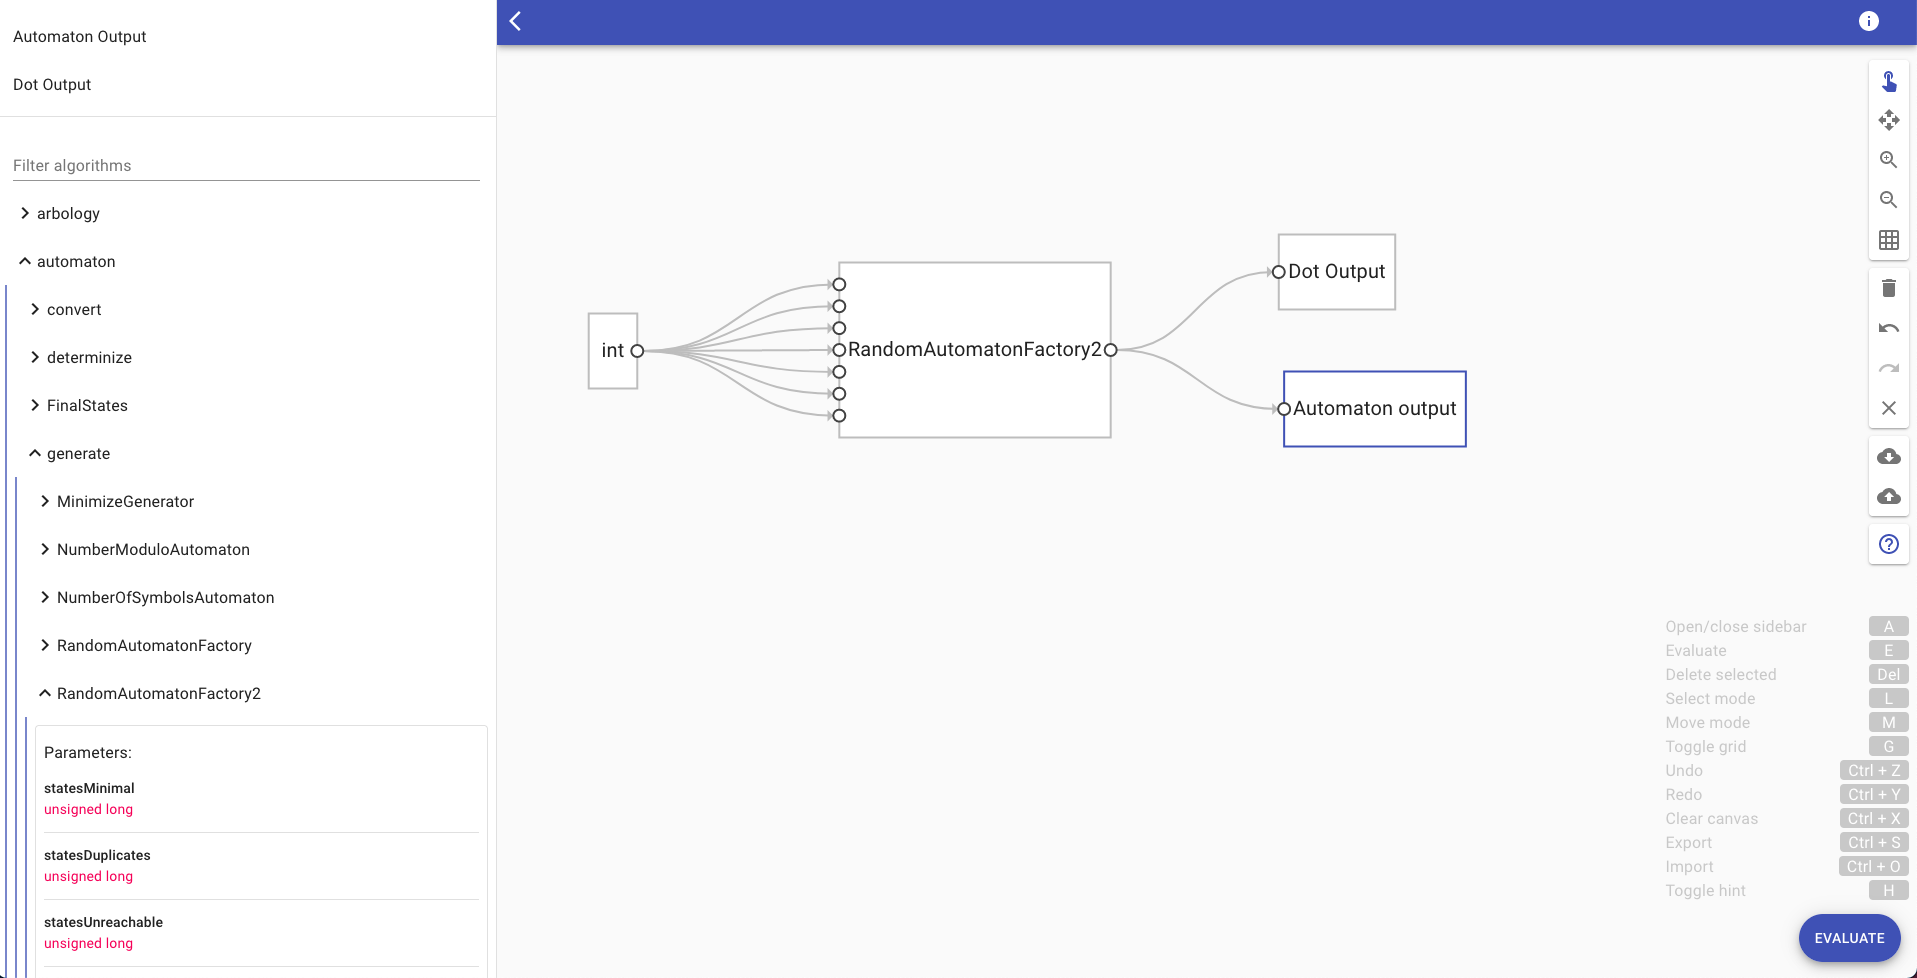
\includegraphics[width=\textwidth]{alt-web-interface}
    \caption{ALT web interface screenshot}\label{alt-web-interface-screen}
\end{figure}

This finite automata editor is called Statemaker and you can see a screenshot of how it looks in figure \ref{statemaker-screen}. To summarize its capabilities - users can:
\begin{itemize}
    \item add states, as well as initial and final states
    \item add transitions between states
    \item edit transition string
    \item mark state as initial or final
    \item remove states and transitions
    \item import and export automaton in supported formats
    \item automatic positioning of transitions and states
\end{itemize}
All of the above features work reliably and are done in intuitive manner - user can quickly understand how to work with all the components. The most notable missing feature is easy simulation of input - this can be done via ALT web interface but if someone is looking for only editing FAs and simulating whether input string is accepted, they have to transition between two interfaces. The benefit is that they can then tap into all the other funcionality that ALT offers. The author of Statemaker has chosen React and Typescript as underlying technologies \cite{state-maker}.

\begin{figure}
    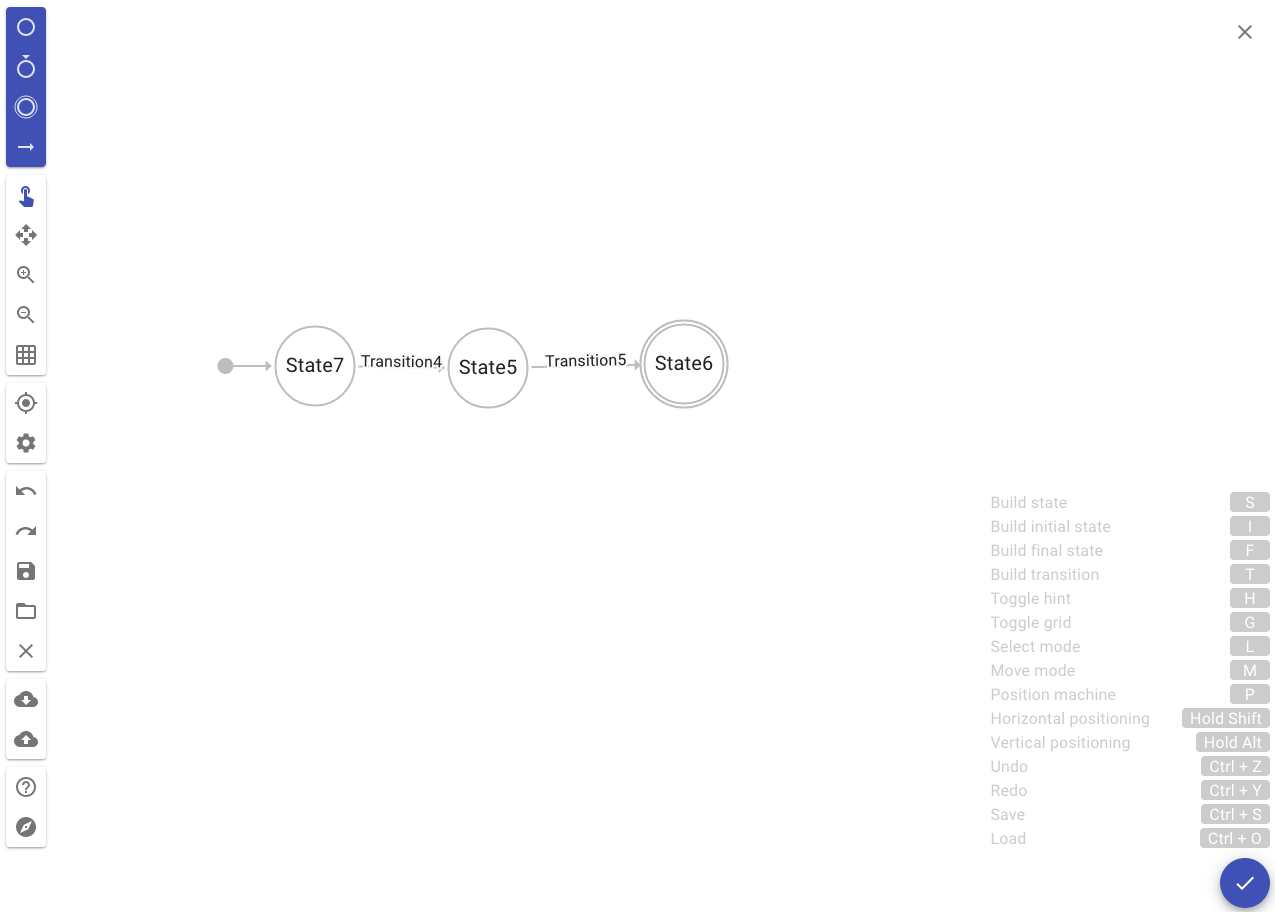
\includegraphics[width=\textwidth]{statemaker}
    \caption{Statemaker screenshot}\label{statemaker-screen}
\end{figure}

\subsection{Existing Applications}

As the main goal of this thesis is to write a finite automata editor for iPad, in this part I will study existing applications mainly for touch devices. 

One of such applications is TuringSim \cite{turingsim}. Although, it is not for FAs but for a Turing machine, it also consists of an editor where user can add and edit states and transitions, thus making it similar to a FA editor. You can see its interface in figure \ref{turingsim-screen}. This editors lets users add and edit automaton's states and transitions. Users can also simulate input on the Turing machine's read-and-write tape. Editing of the automaton is done only via tap gestures which is similar to Statemaker with the difference that there are no distinct buttons for those actions. Therefore, it does not fully utilize the potential of touch devices as the UX is very similar to what would one experience on the web. Unfortunately, the app on iPad is broken at the moment as it is missing bottom toolbar for simulating input.

There is also app called Finite Automata \cite{finite-automata-app}. In this app user can not edit automata in their weighted graph representation but instead has to use a command line that takes individual command which are described in the app. This app does not utilize touch device features at all.

There are also apps available as desktop applications. One is a Finite Automaton Editor by Jaime Rangel-Mondragon that is available as interactive Wolfram notebook \cite{wolfram-editor}. This app allows you to edit the automaton via a transition table and does not allow to simulate any input. There is also Automata Editor by Max Shawabkeh \cite{automata-editor-max}. In this desktop applications users can create and edit their automaton either via a table representation or regular expression. There are also features such as NFA determinization, evaluating automata on strings, and minimizing DFA. Thus it has a powerful feature set but one has to be already familiar with FA theory. It should also be noted that the feature set is a subset of what ALT web interface offers.

\begin{figure}
    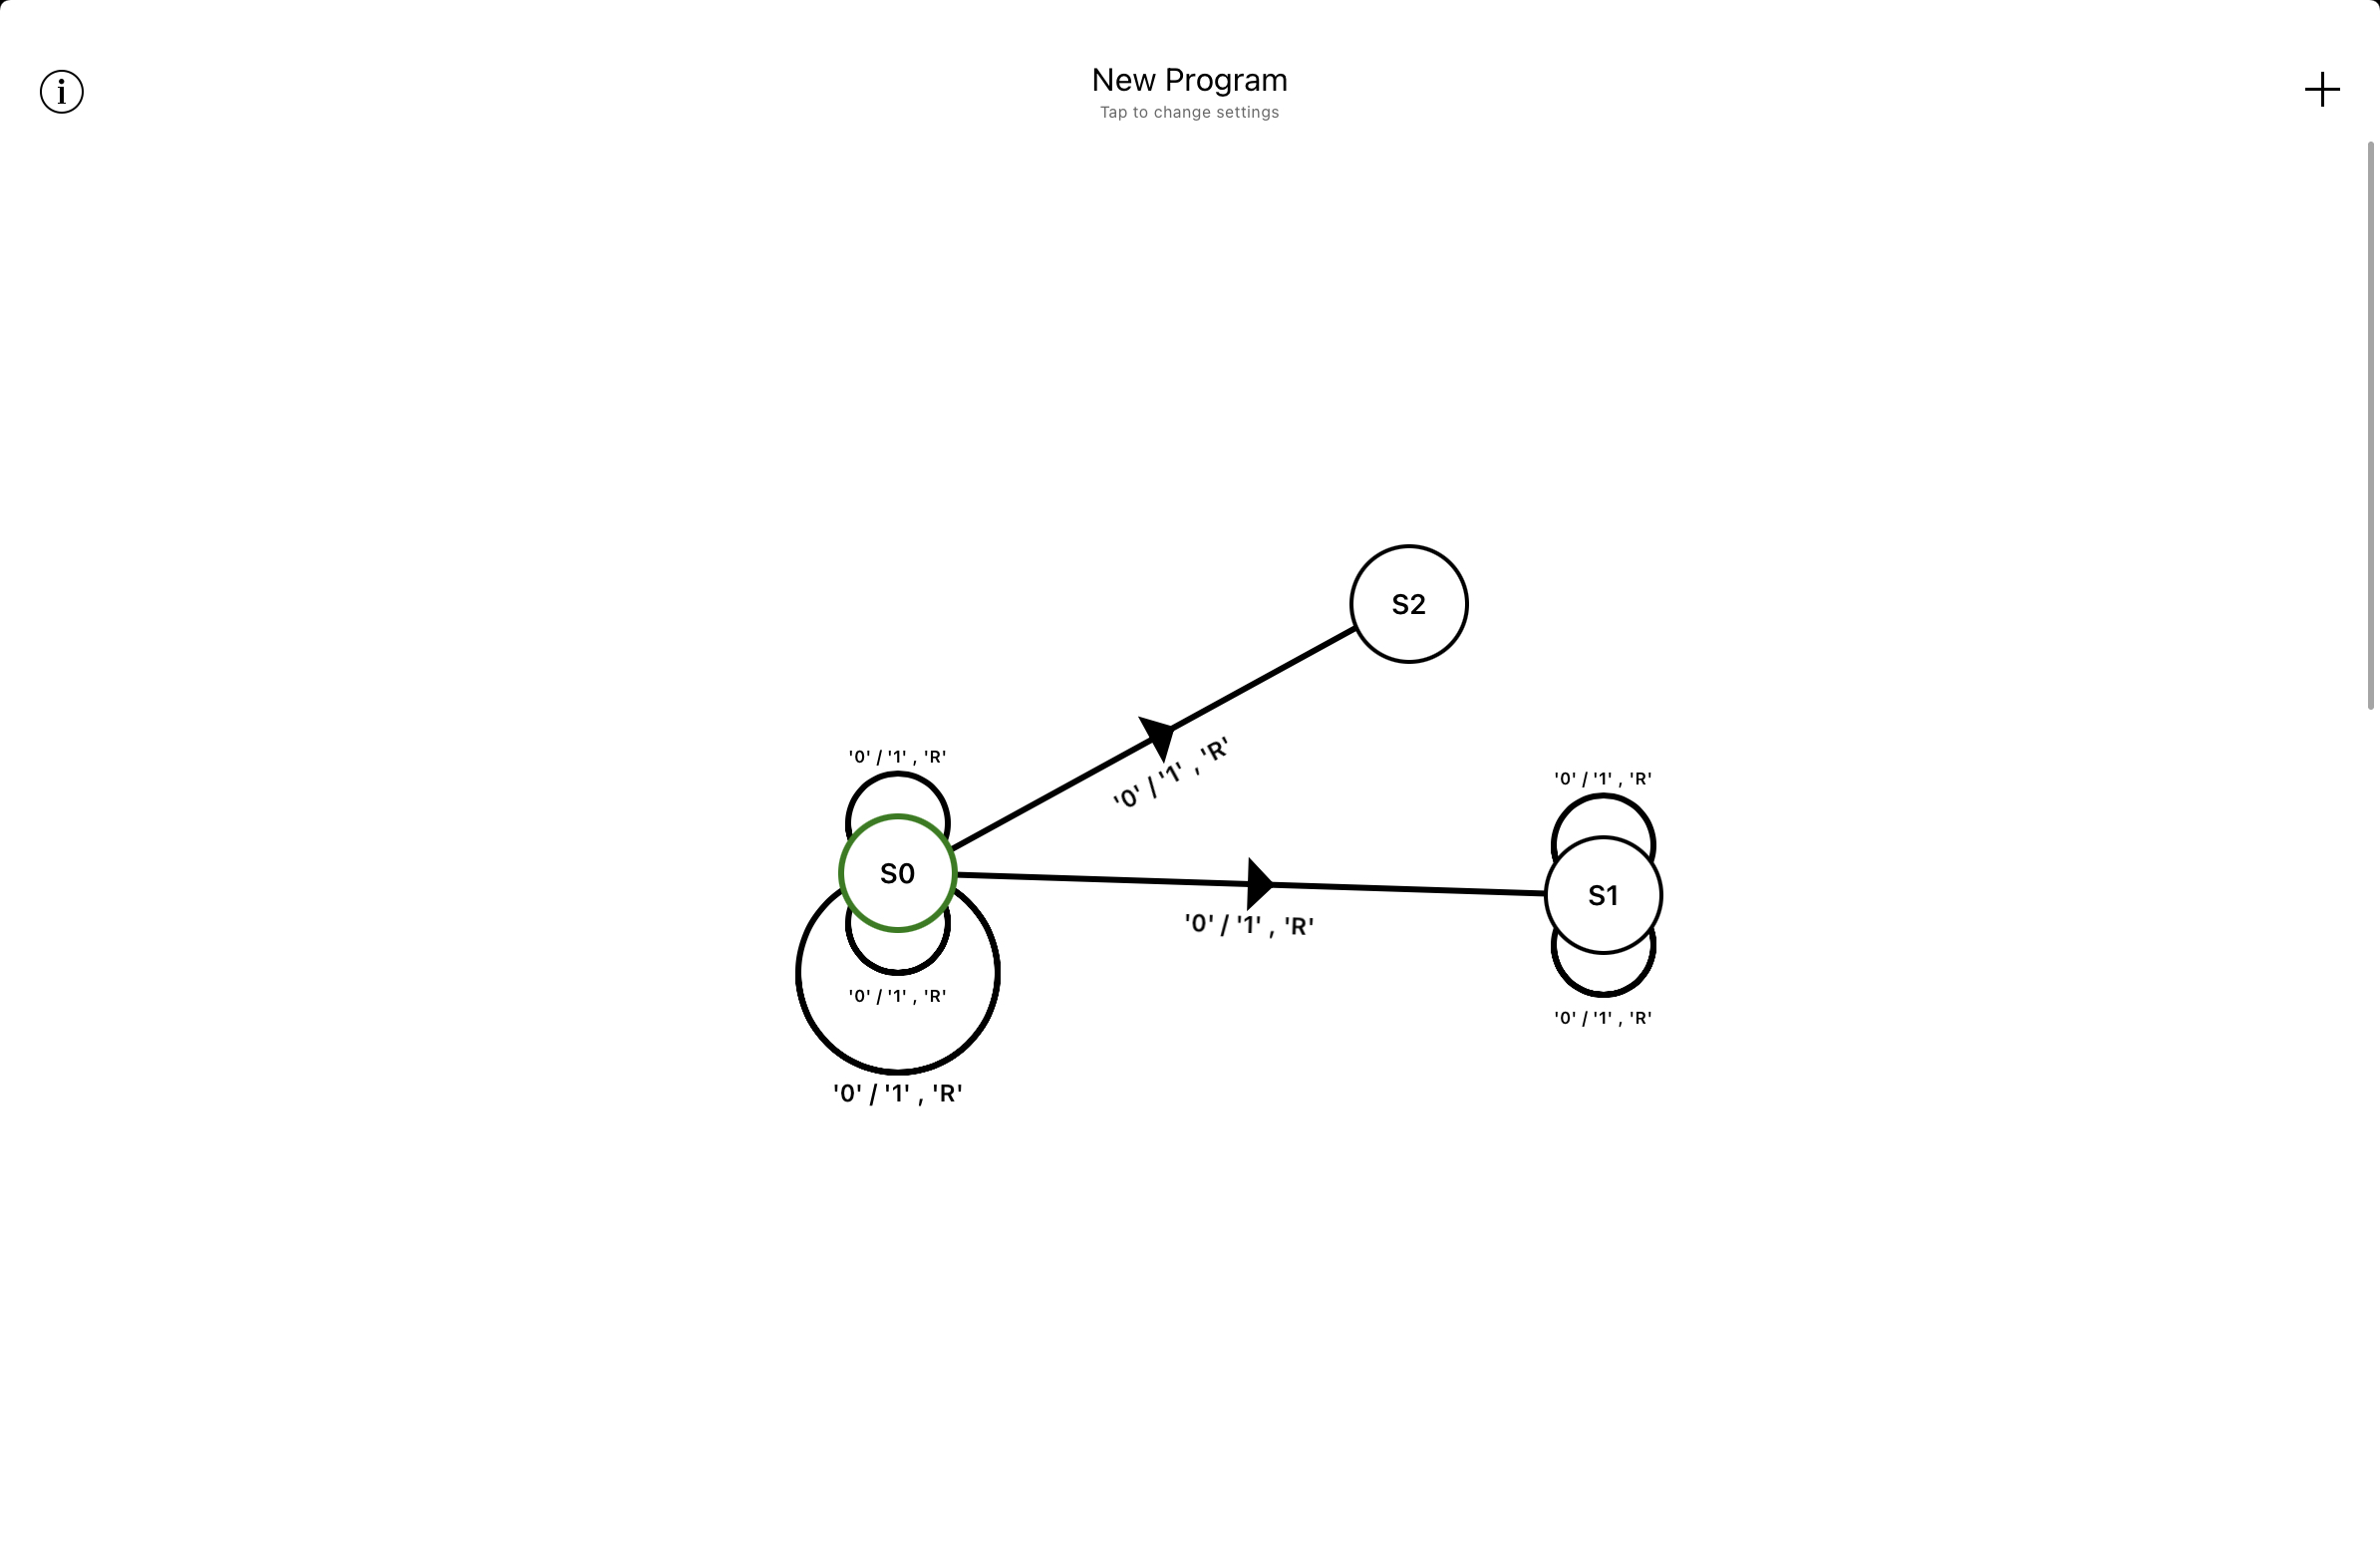
\includegraphics[width=\textwidth]{turingsim}
    \caption{TuringSim interface screenshot}\label{turingsim-screen}
\end{figure}

\chapter{Automata Editor Design}
\label{chap:design}

\chapter{Implementation}
\label{chap:implementation}

\chapter{User Testing}

\chapter{Conclusion}

\section{Goals Assessment}

Assess my goals.

\section{Thesis Contribution}

The contribution of this thesis is testing Algorithms Library Toolkit in practice and can now be pointed to for users who want to see its capabilities. The editor can now also be recommended in the course of BI-AAG at FIT CTU (and other universities) - for students and teachers alike.

\section{Future Work}

Algorithms Library Toolkit is an extensive library and there are still capabilites that are not implemented in the editor.

The choice of developing a native iOS application has resulted in good UX, but in the future it would be beneficial to broaden the possible audience and either develop a similar Android app or create a more ubiquituous web interface.
